%!TEX root = ../AdvMathLecture.tex
%
% Section 10.4: Green's Theorem
% 

%%~~~~~~~~~~~~~~~~~~~~~~   []   ~~~~~~~~~~~~~~~~~~~~~~~~~~~
%\begin{frame}
%\frametitle{\Large {\color[rgb]{0.02,0.20,1.0} \UL{Green's Theorem}}}
%\scriptsize
%
%\begin{block}{Key Concepts:}
%%-------LIST---------
%\begin{itemize}
%	\item[...] Green's Theorem
%\end{itemize}
%%-------------------
%\end{block}
%
%\vspace{1.2cm}
%
%\begin{block}{Mathematical Tools:}
%%-------LIST---------
%\begin{itemize}
%	\item[...] Computing Line Integral using Green's Theorem
%	\item[...] Computing Area using Green's Theorem
%\end{itemize}
%%------------------- 
%\end{block}
%
%%\vspace{3.0cm}
%\end{frame}

\begin{frame}
\frametitle{Topic: Green's Theorem}
\begin{columns}\begin{column}{12.0cm}
\UL{I. Introduction}

\scriptsize

%\UL{Notation}: 

\vspace{0.2cm}

In this section we will on line integrals over closed curves in the $x,y-$plane.
 
\vspace{0.2cm}

{\setlength{\extrarowheight}{-0.1cm}
\begin{tabular}{p{0.85cm}p{11.6cm}}
	\UL{Notation}: & When representing a line integral over a closed curve, we will use the notation
 \\
	&\\
	\multicolumn{2}{c}{\ON<3->{\B{$\OWORK$}} \quad instead of \quad $\WORK$} \\
\end{tabular}}

\vspace{0.2cm}

\begin{center}
	
\includegraphics[scale = 0.25]{\FIGSDIR/10_5_Fig2.png}\\
	Boundary of $R$ is the Closed Curve $C$
\end{center}

\vspace{0.2cm}

{\setlength{\extrarowheight}{-0.1cm}
\begin{tabular}{p{0.45cm}p{11.6cm}}
	\UL{Note}: & Any planar closed curve can be thought of as the boundary of a region, $R$, in the plane.\\
	&\\
\end{tabular}}

\end{column}\begin{column}{0.0cm}\end{column}\end{columns}
\end{frame}

\begin{frame}
\begin{columns}\begin{column}{12.0cm}

\scriptsize

\begin{columns}
\begin{column}{6.0cm}
	\centering
	${\bf F}$ -- Vector Field (Arrows)
	\only<1>{
\includegraphics[scale = 0.3]{\FIGSDIR/10_5_Fig3.png}}
	\only<2>{
\includegraphics[scale = 0.3]{\FIGSDIR/10_5_Fig10.png}}
	\only<3->{
\includegraphics[scale = 0.3]{\FIGSDIR/10_5_Fig11.png}}
\end{column}
\begin{column}{4.5cm}
	
	For the rest of this section, the curves that we will consider have the property of being 
	\ON<2->{\B{simple, closed curves.}}
	
	\vspace{0.3cm}
	
	\DEF A curve is said to be 
	\ON<4->{\B{\,\,{\bf simple}\,\,}} if it never 
	\ON<5->{\B{\,\, crosses itself.}}
	
	\vspace{0.3cm}
	
	\only<1-5>{
\includegraphics[scale = 0.2]{\FIGSDIR/10_5_Fig7.png}}
	\only<6>{
\includegraphics[scale = 0.2]{\FIGSDIR/10_5_Fig8.png}}
	\only<7>{
\includegraphics[scale = 0.2]{\FIGSDIR/10_5_Fig9.png}}
	\only<8->{
\includegraphics[scale = 0.2]{\FIGSDIR/10_5_Fig6.png}}
\end{column}
\end{columns}

\vspace{0.4cm}

{\setlength{\extrarowheight}{-0.1cm}
\begin{tabular}{p{0.15cm}p{11.6cm}}
	\UL{Q}: & Is there a relationship between the region, $R$, the boundary, $C$, and vector field, ${\bf F}$? \\
	&\\
	\UL{A}: & \only<9->{\B{Yes and Green's Theorem provides the answer.}} \\
	&\\
\end{tabular}}

\end{column}\begin{column}{0.0cm}\end{column}\end{columns}
\end{frame}

%%\begin{frame}
%%\scriptsize
%\begin{columns}
%\begin{column}{12.0cm}
%
%\EX	If ${\bf F} = [M, N]$, compute \quad curl$({\bf F}) \cdot {\bf k}$
%
%\vspace{0.2cm}
%
%\SOL
%
%\vspace{8.2cm}
%
%\end{column}
%\begin{column}{0.0cm}\end{column}
%\end{columns}
%\end{frame}

\begin{frame}
\begin{columns}\begin{column}{12.0cm}

\vspace{0.1cm}

\UL{II. Green's Theorem}

\scriptsize

\begin{center}
{\setlength{\extrarowheight}{-0.1cm}
\begin{tabular}{|p{0.4cm}p{10.6cm}|}
	\hline
	\hline
	&\\
	\THM & Let $C$ is a simple closed curve bounding a planar region $R$.  If ${\bf F}(x,y) = [M, N]$ is a vector field, then \\
	&\\
	\multicolumn{2}{|c|}{(General Form) \qquad $\D{\OWORK = 
	\ON<2->{\B{\GINT}}}$} \\
	& \\
	& Since $\D{{\bf F} = 
	\ON<3->{\B{\,[M,N]}}}$, a quick calculation shows: $\D{(\text{curl}\,{\bf F})\cdot {\bf k} = 
	\ON<4->{\B{\,\frac{\PP N}{\PP x}-\frac{\PP M}{\PP y}}\,\,}}$, we have: \\
	& \\
	\multicolumn{2}{|c|}{(Component Form) \qquad $\D{\GREENSL = 
	\ON<5->{\B{\, \GREENSA}}}$} \\
	\hline
	\hline
\end{tabular}}
\end{center}

\begin{center}
	
\includegraphics[scale = 0.24]{\FIGSDIR/10_5_Fig2.png}
\end{center}

\end{column}\begin{column}{0.0cm}\end{column}\end{columns}
\end{frame}

%%\begin{frame}
%\begin{columns}\begin{column}{12.0cm}
%
%\vspace{0.1cm}
%
%\UL{III. Forms of Green's Thm}
%
%\scriptsize
%
%\vspace{0.1cm}
%
%\begin{columns}
%\begin{column}{5.4cm}
%Tangential Form:
%
%\vspace{0.1cm}
%
%{\centering
%$\D{\GREENT = \GREENCURL }$
%}
%
%\vspace{0.2cm}
%
%${\bf T}$ is the unit tangent vector along $C$.
%
%\vspace{0.2cm}
%
%Quantifies the tendency of the vector field to act in the direction of the boundary (circulation).
%
%\vspace{0.2cm}
%
%
\includegraphics[scale = 0.25]{\FIGSDIR/10_5_Fig3.png}
%\end{column}
%\begin{column}{5.4cm}
%Normal Form:
%
%\vspace{0.1cm}
%
%{\centering
%$\D{\GREENN = \GREENDIV }$
%}
%
%\vspace{0.2cm}
%
%${\bf N}$ is the unit normal vector along $C$.
%
%\vspace{0.2cm}
%
%Quantifies the tendency of the vector field to act perpendicularly to the boundary ($flux$).
%
%\vspace{0.2cm}
%
%
\includegraphics[scale = 0.25]{\FIGSDIR/10_5_Fig3.png}
%\end{column}
%\end{columns}
%
%\end{column}\begin{column}{0.0cm}\end{column}\end{columns}
%\end{frame}
%
%%\begin{frame}
%\begin{columns}\begin{column}{12.0cm}
%
%\scriptsize
%Before verifying these lets summarize some notation:
%
%\vspace{0.2cm}
%
%(i) \, $\D{\RPT 
%\ON<2->{\B{\, = [x'(t),y'(t)]}}}$ \quad
%(ii) \,  $\D{{\bf T} 
%\ON<3->{\B{\, = \frac{{\bf r}'(t)}{|{\bf r}'(t)|}}}}$  \quad
%(iii) \, $\D{{\bf N} 
%\ON<4->{\B{\, ={\bf T} \times {\bf k}}}}$  \quad
%(iv) \, $\D{d{\bf r} 
%\ON<5->{\B{\,= \RPT \, dt}}}$  \quad
%(v) \, $\D{ds 
%\ON<6->{\B{\,= |\RPT| \, dt}}}$
%
%\vspace{0.2cm}
%
%Tangential Form: \quad $\D{\GREENT = \GREENCURL }$
%%--------EQN----------
%\begin{align*}
%	\GREENT = 
%	\ON<7->{\B{\, \oint \limits_{C} {\bf F} \cdot \frac{\RPT}{|\RPT|}\, (|\RPT|\,dt)}}
%	\ON<8->{\B{\,= \oint \limits_{C} {\bf F} \cdot \RPT\,dt}}
%	\ON<9->{\B{\,= \oint \limits_{C} {\bf F} \cdot d{\bf r}}}
%	\ON<10->{\B{\,= \GREENCURL \quad \checkmark}}
%\end{align*}
%%----------------------
%Normal Form: \quad $\D{\GREENN = \GREENDIV}$
%%--------EQN----------
%\begin{align*}
%	(*)\quad{\bf N}\,ds = ({\bf T} \times {\bf k})\, ds
%\ON<11->{\B{ \,= \left(\frac{\RPT}{|\RPT|} \times {\bf k}\right)\, (|\RPT|\,dt)}}
%&\ON<12->{\B{\,= \frac{1}{|\RPT|}\left(\RPT \times {\bf k}\right)\, (|\RPT|\,dt)}}\\
%&\ON<13->{\B{ \,= \left(\RPT \times {\bf k}\right)\,dt}}\\
%&\ON<14->{\B{ \,= \left([x'(t),y'(t),0] \times [0,0,1]\right)\, dt}}\\
%&\ON<15->{\B{ \,= \left[y'(t),-x'(t),0\right]\, dt}}\\
%&\ON<16->{\B{ \,= \left[\frac{dy}{dt},-\frac{dx}{dt},0\right]\, dt}}\\
%&\ON<17->{\B{ \,= [dy,-dx,0]}}\\
%&\ON<18->{\B{ \,= [dy,-dx]}}
%\end{align*}
%%----------------------
%\end{column}\begin{column}{0.0cm}\end{column}\end{columns}
%\end{frame}
%
%%\begin{frame}
%\begin{columns}\begin{column}{12.0cm}
%
%\scriptsize
%and so, by (*), we have ...
%%--------EQN----------
%\begin{align*}
%	\ON<2->{\B{\GREENN = }}
%	\ON<3->{\B{\, \oint \limits_{C} {\bf F} \cdot ([dy,-dx])}}
%	&\ON<4->{\B{\,\,= \oint \limits_{C} [M,N] \cdot [dy,-dx]}}\\
%	&\ON<5->{\B{\,\,= \oint \limits_{C} M\, dy - N \, dx}}\\
%	&\ON<6->{\B{\,\,= \oint \limits_{C} - N \, dx + M\, dy }}\\
%	&\ON<7->{\B{\,\,= \iint \limits_{R} (M)_x - (-N)_y\,dA }}\\
%	&\ON<8->{\B{\,\,= \iint \limits_{R} M_x + N_y \,dA }}\\
%	&\ON<9->{\B{\,\,= \GREENDIV \quad \checkmark}}\\
%\end{align*}
%%----------------------
%
%\vspace{6.2cm}
%	
%\end{column}\begin{column}{0.0cm}\end{column}\end{columns}
%\end{frame}

\begin{frame}
\begin{columns}\begin{column}{12.0cm}

\scriptsize

\EX Let $\D{{\bf F} = [x^2 + 4y, x + y^2]}$ and let \,\, $C$ be a square bounded by: \,\, $x=0$, $x=1$, $y=0$, and $y=1$,

\vspace{0.2cm}

Compute \quad $\D{\OWORK}$

\vspace{0.2cm}

To compute this directly we would have to compute 
\ON<2->{\B{a line integral for $C_1$, $C_2$, $C_3$, and $C_4$}}

\begin{columns}
\begin{column}{7.5cm}

\vspace{0.3cm}

$\D{\OWORK = 
\ON<3->{\B{\oint \limits_{C_1} \FDR + \oint \limits_{C_2} \FDR + \oint \limits_{C_3} \FDR + \oint \limits_{C_4} \FDR}}}$

\vspace{0.3cm}

\ON<2->{\B{and we would need to parameterize (\,find $\RT$\,) all 4 curves}}

\vspace{0.3cm}

\ON<4->{\B{Alternatively, we could apply Green's Theorem}}

\vspace{0.3cm}

\ON<4->{\B{$\D{\OWORK = \GREENSA}$}}

\vspace{0.4cm}

$\D{
\ON<5->{\B{\frac{\partial N}{\partial x} = 1}}}$ \quad 
\ON<6->{\B{and}} \quad $\D{
\ON<7->{\B{\frac{\partial M}{\partial y} = 4}}}$

\vspace{0.4cm}

$\D{ 
\ON<8->{\B{\OWORK = \iint \limits_{R} (1-4)\, dA =\,}} 
\ON<9->{\B{-3 \iint \limits_{R} \, dA =\,}}
\ON<10->{\B{-3 \, (Area \, of \, R) = -3}}}$

\end{column}
\begin{column}{3.3cm}

\only<1>{
\includegraphics[scale = 0.19]{\FIGSDIR/10_5_Fig5.png}}
\only<2->{
\includegraphics[scale = 0.19]{\FIGSDIR/10_5_Fig4.png}}
	
\end{column}
\end{columns}

\vspace{0.6cm}

\end{column}\begin{column}{0.0cm}\end{column}\end{columns}
\end{frame}

\begin{frame}
\begin{columns}\begin{column}{12.0cm}

\scriptsize

\EX Let $\D{{\bf F} = [16xy + 3yx^2, x^3 + 2y]}$ and let \,\, $C$ be a triangle bounded by: \,\, $x=3$, \, $y=0$, and $y=x$

\vspace{0.2cm}

Compute \quad $\D{\OWORK}$

\vspace{0.2cm}

First compute: \quad
$\D{
\ON<2->{\B{N_x = (x^3 + 2y)_x }}
\ON<3->{\B{\,= 3x^2}}
}$
\hspace{1.0cm} 
\ON<3->{\B{and}} \hspace{1.0cm}
$\D{
\ON<4->{\B{M_y = (16xy + 3yx^2)_y}}
\ON<5->{\B{\,= 16x + 3x^2}}
}$
\vspace{0.2cm}
\begin{columns}
\begin{column}{6.0cm}
\ON<6->{\B{and apply Green's Thm:}}
%--------EQN----------
\begin{align*}
	\ON<7->{\B{\OWORK}}
	&\ON<7->{\B{\, = \iint \limits_{R} (3x^2)-(16x + 3x^2)\, dA }}\\
	&\ON<8->{\B{\,=\, \iint \limits_{R} -16x\, dA }}\\
	&\ON<11->{\B{\,=\, \int \limits_{0}^{3}\int \limits_{0}^{x} -16x\, dydx }}\\
	&\ON<12->{\B{\,=\, \int \limits_{0}^{3} \left.-16xy\right|_{y=0}^{y=x} \, dx }}\\
	&\ON<13->{\B{\,=\, \int \limits_{0}^{3} -16x^2 \, dx }}
	\ON<14->{\B{\,=\, \left.-\frac{16}{3}x^3\right|_{0}^{3} }}
	\ON<15->{\B{\,\,=\, -\frac{16}{3}(3)^3 = -144}}
\end{align*}
%----------------------	
\end{column}
\begin{column}{4.0cm}
	\ON<9->{\B{Plot the region bounded by $C$:}}
	
	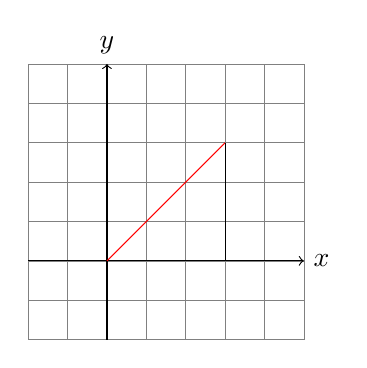
\begin{tikzpicture}[x=0.5cm,y=0.5cm]

  		\def\xmin{-2}
		\def\xmax{5}
		\def\ymin{-2}
		\def\ymax{5}

		  % grid
  		\draw[style=help lines, ystep=1, xstep=1] (\xmin,\ymin) grid
  		(\xmax,\ymax);

  		% axes
  		\draw[->] (\xmin,0) -- (\xmax,0) node[right] {$x$};
  		\draw[->] (0,\ymin) -- (0,\ymax) node[above] {$y$};

  		% xticks and yticks
  		%\foreach \x in {-2,-1,...,5}
    		%\node at (\x, \ymin) [below] {\x};
  		%\foreach \y in {-2,-1,...,5}
    		%\node at (\xmin,\y) [left] {\y};

  		% plot the data from the file data.dat
  		% smooth the curve and mark the data point with a dot
%  		\draw[color=blue] plot[smooth,mark=*,mark size=1pt] file {data.dat}
%   		node [right] {data};

  		% generate and plot another a curve y = 0.1 x^2 + 2.5
  		% this generates the files figure.parabola.gnuplot and figure.parabola.table 
  		\ON<10->{\B{\draw[color=red, domain=0:3] plot (\x, {\x});}}
		\ON<10->{\B{\draw[-] (3,0) -- (3,3);}}
  		%function{x} node [right] {$y=0.1\,x^2 + 2.5$};

\end{tikzpicture}
	
\end{column}
\end{columns}

\vspace{7.2cm}

\end{column}\begin{column}{0.0cm}\end{column}\end{columns}
\end{frame}

\begin{frame}
\begin{columns}\begin{column}{12.0cm}

\scriptsize

\EX Let $\D{{\bf F} = [xy, y^2]}$ and let \,\, $R$ be the region in the first quadrant bounded by:\, $y=x^2$, \, and \, $y=x$

\vspace{0.2cm}

Compute \quad $\D{\OWORK}$

\vspace{0.2cm}

\vspace{7.2cm}

\end{column}\begin{column}{0.0cm}\end{column}\end{columns}
\end{frame}

\begin{frame}
\begin{columns}\begin{column}{12.0cm}

\scriptsize

\EX Let $\D{{\bf F} = \nabla(x^2\sin y)}$ and let\, $R$ be the region bounded by: \,\, $x=1$, \, $y=0$, \, and \, $y=\sqrt{x}$

\vspace{0.2cm}

Compute \quad $\D{\OWORK}$

\vspace{0.2cm}

\vspace{7.2cm}

\end{column}\begin{column}{0.0cm}\end{column}\end{columns}
\end{frame}


\begin{frame}
\frametitle{Summary: Line Integral over Vector-Valued Functions}
\begin{columns}\begin{column}{12.0cm}

\scriptsize

\vspace{0.1cm}

We have 3 main methods for computing line integrals over a vector-valued function ${\bf F}$:
%-------NUM LIST---------
\begin{enumerate}
	\item[(1)] Directly 
	\ON<2->{\B{$\D{\left[\text{i.e. find } \RT \,\, \text{and compute} \,\, \WORKT \right]}$}}
	\item[(2)] Fundamental Thm of Line Integrals 
	\ON<3->{\B{$\D{\left[\text{i.e. find } f \,\, \text{s.t. } \,\, \nabla f = {\bf F} \,\, \implies \,  \WORKAB = f(B)-f(A) \right]}$}}
	\item[(3)] Green's Thm 
	\ON<4->{\B{$\D{\left[\text{i.e. apply} \,\, \WORK = \iint \limits_{R} (N_x - M_y)\, dA \right]}$}}
\end{enumerate}
%------------------------
%--------TABLE---------
\begin{table}
	\setlength{\extrarowheight}{0.01cm}
	\begin{tabular}{| c | c | c | c |}
		\hline
		C closed? & $\D{\bf F}$ Conservative? (curl ${\bf F} = {\bf 0}$?) & Use Method & {\bf r} \, needed?\\
		\hline
		\multirow{4}{*}{Yes} & \multirow{2}{*}{Yes} & 	\multirow{2}{*}{
			\ON<5->{\B{$\D{\int_{C} {\bf F}\cdot d{\bf r} = 0}$}}} & \multirow{2}{*}{No}\\
		&&&\\
		\cline{2-4}
		    & \multirow{2}{*}{No} & \multirow{2}{*}{
		    \ON<6->{\B{(3)}}} & \multirow{2}{*}{No}\\
		&&&\\
		\hline
		\multirow{4}{*}{No} & \multirow{2}{*}{Yes} & \multirow{2}{*}{
			\ON<7->{\B{(2)}}} & \multirow{2}{*}{No}\\
		&&&\\
		\cline{2-4}
		    & \multirow{2}{*}{No} & \multirow{2}{*}{
		    \ON<8->{\B{(1)}}} & \multirow{2}{*}{Yes}\\
		&&&\\
		\hline
	\end{tabular}
\end{table}
%--------------------
Note: Method (1) can always be applied to any line integral
\end{column}\begin{column}{0.0cm}\end{column}\end{columns}
\end{frame}

%%\begin{frame}
%\frametitle{Surface Integrals: Vector-Valued Functions}
%\scriptsize
%\begin{columns}
%\begin{column}{12.0cm}
%
%\vspace{0.1cm}
%
%We have 3 main methods for computing surface integrals over a vector-valued function ${\bf F}$:
%%-------NUM LIST---------
%\begin{enumerate}
%	\item[(1)] Directly - version 1:
%	\ON<2->{\B{$\D{\left[\text{i.e. find } {\bf r}(u,v) \,\, \text{and compute} \,\,  \FLUXXX \right]}$}}
%	\item[(2)] Directly - version 2:
%	\ON<2->{\B{$\D{\left[\text{i.e. determine } {\bf n} \,\, \text{and compute} \,\, \FLUXX \right]}$}}
%	\item[(3)] Divergence Thm 
%	\ON<4->{\B{$\D{\left[\text{i.e. apply} \,\, \FLUX = \DIVTHM \right]}$}}
%\end{enumerate}
%%------------------------
%%--------TABLE---------
%\begin{table}
%	\setlength{\extrarowheight}{0.01cm}
%	\begin{tabular}{| c | c | c | c |}
%		\hline
%		S closed? & {\bf n} \, known? & Use Method & {\bf r} \, needed?\\
%		\hline
%		\multirow{4}{*}{Yes} & \multirow{2}{*}{Yes} & \multirow{2}{*}{
%			\ON<5->{\B{(3)}}}& \multirow{2}{*}{No}\\
%		&& & \\
%		\cline{2-4}
%		    & \multirow{2}{*}{No} & \multirow{2}{*}{
%		    \ON<6->{\B{(3)}}}& \multirow{2}{*}{No}\\
%		&& & \\
%		\hline
%		\multirow{4}{*}{No} & \multirow{2}{*}{Yes} & \multirow{2}{*}{
%			\ON<7->{\B{(2)}}}& Depends on $S$ and \\
%		&& & the value of ${\bf F} \cdot {\bf n}$ \\
%		\cline{2-4}
%		    & \multirow{2}{*}{No} & \multirow{2}{*}{
%		    \ON<8->{\B{(1)}}}& \multirow{2}{*}{Yes}\\
%		&& & \\
%		\hline
%	\end{tabular}
%\end{table}
%%--------------------
%Note: Method (1) can always be applied to any surface integral 
%\end{column}
%\begin{column}{0.0cm}\end{column}
%\end{columns}
%\end{frame}
%
%%\begin{frame}
%\frametitle{Line and Surface Integrals: Scalar-Valued Functions}
%\scriptsize
%\begin{columns}
%\begin{column}{12.0cm}
%Let $g$ be a scalar-valued function.
%
%\vspace{0.4cm}
%
%Line Integral \,\, - \,\, $C$ is a curve
%
%\begin{center}
%	$\D{\int \limits_{C} g \, ds = 
%	\ON<2->{\B{\int \limits_{a}^{b} g\,({\bf r}) \cdot |{\bf r}'| \, dt }}}$
%\end{center}
%
%\vspace{0.2cm}
%
%Surface Integral \,\, - \,\, $S$ is a surface
%
%\begin{center}
%	$\D{\int \limits_{S} g \, dA = 
%	\ON<4->{\B{\iint \limits_{R} g({\bf r}) \cdot |{\bf N}| \, du \, dv}}}$
%\end{center}
%
%\vspace{0.5cm}
%
%$R$ is the region in the $u,v$-plane (parameter plane).
%
%\vspace{1.2cm}
%
%\end{column}
%\begin{column}{0.0cm}\end{column}
%\end{columns}
%\end{frame}
